\documentclass{standalone}

\usepackage[latin1]{inputenc}
\usepackage{tikz}
\usetikzlibrary{trees,shapes.multipart}
\begin{document}
\pagestyle{empty}


% Set the overall layout of the tree
\tikzstyle{level 1}=[level distance=11em, sibling distance=10ex]

% Define styles for bags and leafs
\tikzstyle{bag} = [rectangle, draw, text width=10em, text centered, thick]

% The sloped option gives rotated edge labels. Personally
% I find sloped labels a bit difficult to read. Remove the sloped options
% to get horizontal labels.
\begin{tikzpicture}[edge from parent/.style={draw,-latex},very thick]
\node[circle,draw,inner sep=1.5] {Початок $\varepsilon_0$}
  child[grow=left] {
    node[bag] {
      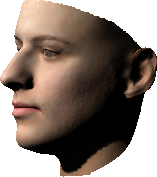
\includegraphics[width=0.45\textwidth]{../images/trees/profile}
      \\
      Профіль
      $\left\langle t^2, \theta^2 \right\rangle$
    }
  }
  child[grow=down] {
    node[bag] {
      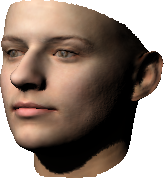
\includegraphics[width=0.45\textwidth]{../images/trees/3-4}
      \\
      Три чверті
      $\left\langle t^3, \theta^3 \right\rangle$
    }
  }
  child[grow=right] {
    node[bag] {
      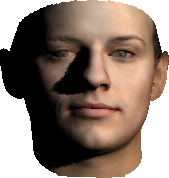
\includegraphics[width=0.45\textwidth]{../images/trees/frontal-shaded}
      \\
      Анфас з боковим освітленням
      $\left\langle t^4, \theta^4 \right\rangle$
    }
  }
  child[grow=up] {
    node[bag] {
      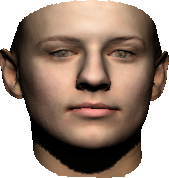
\includegraphics[width=0.45\textwidth]{../images/trees/frontal}
      \\
      Анфас
      $\left\langle t^1, \theta^1 \right\rangle$
    }
  };
\end{tikzpicture}

\end{document}
